\section{Visual Target Selection Emerges from a Bio-inspired Network Topology}
\begin{center}
Wahiba Taouali, Nicolas Rougier et Fr\'ed\'eric Alexandre\\
Studies in Computational Intelligence, pages 317--330.\\
\end{center}


\paragraph{Abstract}
%The abstract should summarize the contents of the paper and should
%contain at least 70 and at most 150 words. It should be written using the
%\emph{abstract} environment.

 \textit{The orientation of sensors toward regions of interest of the
  environment is an important motor activity, monitored by ancient
  structures of the brainstem. Particularly, the superior colliculus
  is known to be deeply involved in visual saccadic behavior. Target
  selection relies on various hints including exogenous information
  about the nature and the position of candidate targets and
  endogenous information about current motivations. We present a model
  of the collicular structure based on biological data, the
  specificity of which is related to the homogeneity of the underlying
  substratum of computation. This makes it more suitable to process
  massive visual flows on a distributed architecture, as it could be
  requested in a realistic task in autonomous robotics. The present
  model is restricted to the exogenous part of the visual pathway,
  from the retina to the superior colliculus. A realistic behavior for
  the selection of exogenous targets is reported here.}

%---------------------------------------------------------------------------

\subsection{Introduction}

Displaying an intelligent behavior is often synonymous of
intelligently exploiting the surrounding environment. In many animals,
this is massively performed through the analysis of information by the
visual channel, to orient subsequent behavior (perceptual decision and
action). Much research in computational intelligence aims at endowing
animats with such powerful skills, drawing inspiration from the living
science, at several levels of description. At the functional level, it
is important to know which information animals extract from the visual
input, possibly in parallel communicating processing flows and,
accordingly, which representations are built and exploited in memory
systems. At the physiological level, if one wishes a deep anchoring in
biological inspiration, the functional behavioral analysis has to be
mapped onto the neural substratum and its known anatomy and
physiology, which can also give indications about the way behavioral
properties can emerge from fine grained neural computations. At the
operational level, a formalism of computation has to be defined to
implement the corresponding models, as a compromise between accuracy
to biological inspiration and efficiency of computation for animats
plunged in the real world.

\subsubsection{At the functional level}

It has been proposed for a long time \cite{Ungerleider:1982} that two
separate visual systems can be described in the ventral (temporal) and
dorsal (parietal) visual cortex. These associative cortical areas
were first respectively presented as dedicated to identification and
location of objects. Later \cite{Milner:1995}, it was more precisely
explicited that the ventral cortex elaborates the construction of the
perceptive representation of objects in the world, thanks to its
privileged relationships with the limbic system, center of the
declarative memory, whereas the dorsal cortex, linking the primary
visual cortex and the motor cortex, allows for the visual control of
actions towards that objects, by extracting, in the visual flow,
information useful for the preparation of actions (eg. size of an
object for anticipating the size of the grip in a grasping movement). 

In \cite{Goodale:1998}, the authors explain that both cortical axes
are separate but deeply interacting in primates and conclude that this
dual view reconciliates the reconstructionist approach by D. Marr, very
much influential in the domain of computer vision, and the
purposive-animate-behaviorist approach by J. Gibson, very popular in
reactive robotics.  Particularly, the interplay between both
functional analysis is well illustrated by two adaptive behaviors that
allow to decrease the huge amount of information brought by the visual
channel: visual attention proposes a sequential processing of possible
targets; saccadic movements orient the body and particularly the fovea
on regions of interest in the visual scene. In both cases, the visual
control of action is dedicated to elaboration of a flexible and
powerful representation of the visual information. According to
\cite{Ballard:1997}, fixation and attention can be considered as
mechanical and neural deictic devices and the authors explain the
computational power of such a technique for variable binding and other
strategies of embodied representation. At the cerebral level, the
premotor theory of attention \cite{Rizzolatti:1987} stipulates that
there are common processes between these key behaviors and, more
precisely, that they share common neuronal circuits: Attention would
be pre-programming of a saccade.

\subsubsection{At the physiological level}

In the above mentioned paper \cite{Goodale:1998}, the authors also
make a very precious reference to phylogenesis and indicate that, in
more primitive animals, the goal of vision is not to see but to guide
their movements. The visual control of actions corresponds to a direct
instantaneous perception system, whereas the identification of objects
can be seen as a relation from the present visual input to a past
information stored in declarative memory, not present in ancient
species (eg. reptilians, amphibians). Consequently, the general
purpose network that we observe in the brain of primates, where the
cortex plays a major role, must be also related to the basic visual
system of a frog \cite{Lettvin:1968}, where only several input/output
sensorimotor lines (predator avoidance, prey catching, locomotion
guiding) define a kind of purposive vision. The very nature of the
evolution of the brain makes that these ancient visuomotor structures
are still present, though modulated of course by advanced control
systems and coordinated by more recent memory systems.

Particularly, these circuits converge, in the frog, in a neural
structure called the tectum, directly linking retinal inputs to motor
actions. In mammals, the similar structure is called the superior
colliculus (SC).  Indeed, this small structure in the midbrain of
mammals is known to be implicated in these sensorimotor
behaviors. From an hodological viewpoint, it integrates visual
information from many sources (cortical or not) in the brain and sends
projections toward the brainstem premotor circuits that trigger
saccades \cite{Isa:2002}. From an anatomical viewpoint, it consists of
a set of topological maps, mapping the surrounding space, from visual
to motor reference frames \cite{Girard:2005}. And from a physiological
viewpoint, its inactivation or electrical stimulation confirms its
role in visual attention and saccades \cite{Muller:2005}.

Many models have studied the SC and associated properties
(cf. \cite{Girard:2005} for a review). We just mention here some models
underlying the link to information flows and underlying behavior. The structure
of the model described in \cite{Findlay:1999} underlines that the main task is
to decide when and where the saccade must be performed. As a consequence, two
hierarchical axes are defined. The When axis (corresponding to the FEF (Frontal
Eye Field) area in the prefrontal cortex) decides when to leave the current
fixation point, whereas the Where axis corresponds to the SC and implements a
spatial competition between candidate targets. A double-axis model combining
FEF and the SC is also proposed in \cite{Kramer:1999}, to explain the
integration of exogenous elements (external stimuli coming from the retina to
the SC) and endogenous elements (internal expectancies or instructions
elaborated in the prefrontal cortex). Later on, \cite{Godijn:2002} proposed a
competitive integration model based on strong experimental evidences at the
behavioral level, indicating that all these elements (spatial vs temporal
processing and integration of exogenous vs endogenous stimuli) can be
integrated in a unique map, seen as a model of the SC. This common saccade map
also includes features generally reported as physiologically plausible in the
SC: a local excitation in the map allowing to combine close stimuli and a wider inhibition mechanism to trigger a competition between far stimuli. This
interaction scheme explains why it was possible to use such a formalism as
Dynamic Neural Field (DNF) \cite{Amari:1977} to implement this kind of model, as it is also the case in \cite{Trappenberg:2001,Schneider:2002}.

\subsubsection{At the operational level}

Many recent models of the SC explain a wider range of visuomotor and more
generally cognitive functions at the price of a more complex internal circuitry
describing the SC. Indeed, those models define several kinds of units,
depending on their location on the map, which is not very consistent with the
principle of homogeneity in DNF. More precisely, in \cite{Trappenberg:2001},
the reported behavior is obtained with some units standing for the currently
fixated stimulus (consequently in the fovea), other units representing
potentially fixated stimuli in the periphery, both kinds sending inhibition to
other units triggering saccades toward a target. These kinds of units, also
exploited in the model by \cite{Schneider:2002}, are presented as representing
respectively so-called fixation, build-up and burst neurons, which are
sometimes reported as parts of the intermediate layer of the SC
\cite{Wurtz:1994}, though this is still to be clearly established. In
\cite{Godijn:2002} also, the substratum of computation is not homogeneous,
since the sensitivity of units decreases with their eccentricity onto the
map. This trick is used to reproduce the observation that the latency of a
saccade toward a target, presented together with a distractor, is longer when
the distractor is closer from the rostral zone of the SC (corresponding to the
fovea).

Consequently, these complex models often rely on physiological considerations
that are controversial and their inner mechanisms can often be described as ad
hoc, designed to stick to experimental observations. Moreover, this additional
complexity is often obtained by introducing numerous parameters, which affects negatively the
robustness of these models. Also, it becomes difficult to simulate
on-line the analysis of a visual flow, due to the amount of generated
computations. Such an assessment is contradictory to the ordinary view that
neuronal structures are often homogeneous, due to the repetitive tiling of
elementary circuits of neurons. It is also contradictory to the spirit of DNF
that have been designed as a generic homogeneous model for such populations of
neurons.  For that reasons, in this paper, we present a model of the SC, based
on DNF formalism, with an identical functioning rule for all the units in the
map. Moreover, obtaining such an homogeneous substratum can yield fully
distributed computation, which is important to design models that can be used
online in robotic visuomotor tasks. Also, this approach has a common ground
with the reactive and enactive frameworks mentioned above, which state that
fundamental properties can emerge from low-level, basic computations and not
from a high-level structured module. Correspondingly, one of our questions here
is to observe which of the known properties of the SC we can obtain with such
an homogeneous and simple brick of computation.

Finally, the proposed model is not an isolated structure but is a function of
exogenous information flows and associated geometrical properties.  We have
explained that the SC is undoubtedly an important integrative structure, to be
included in a cognitive neuroscience modeling approach of visuospatial
behaviors and we will illustrate accordingly how this model could be exploited
in more high level tasks.



%---------------------------------------------------------------------------
\subsection{Model}
The computational paradigm supporting the model is grounded on the
notion of a unit that is essentially a set of time dependent values
varying under the influence of other units via learnable weighted
links (fig. \ref{fig:group}).  The evolution of units' value is
defined by a set of differential equations expressed in standard
mathematical notations. The units are organized into groups that form
a network and each unit can be linked to any other unit (including
itself) using a weighted link. The modeling framework\footnote{See
  \url{http://dana.loria.fr}} offers a set of core objects needed to
design and run such networks. However, in this framework, what is
actually computed by a unit and what is learnt are the responsibility
of the modeler who is in charge of providing the equations governing
the unit's behavior and the plasticity of its links.
%%
\begin{figure} %[htbp]
  \begin{center}
    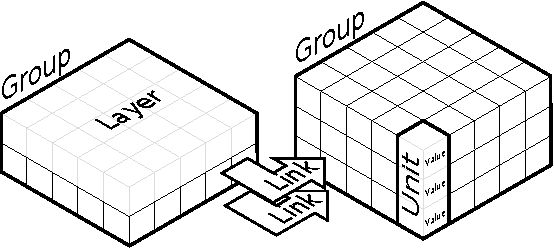
\includegraphics[width=\textwidth]{Chapitres/PublicationsSample/Chapitre/figures/group}
  \end{center}
  \caption {A unit is a set of one to several values ($V_i$). A group is a
    structured set of one to several homogeneous units. A layer is a subset of
    a group restricted to a unique value $V_i$. A layer is a group. A link is a
    weighted connection between a source group to a target group. A group can
    be linked to any other group including itself.}
  \label{fig:group}
\end{figure}
Such a modeling framework is actually strongly constrained and cannot cope for
example with standard artificial neural networks. It is indeed centered around a
set of four principles (distributed, asynchronous, numerical and adaptive) that
we think may help to bring insights on our understanding of computational
intelligence. While many computational models involve explicit symbols and/or
a central supervisor, this framework is able to guarantee to a certain extent
the absence of such artifacts. In the end, what is achieved by such a model is
the sole result of the interaction of many units working together.


\subsubsection{Model architecture}
In short, we consider here projections to the SC coming from the
retina and the primary visual cortex, carrying exogenous information,
and not those coming from the frontal cortex, carrying endogenous
information.  Under that restriction, we want to check to what extent
the model exhibits some of the well known properties of saccadic
behavior associated to the SC. More specifically, our goals are to
analyze the topology of the visual information that we obtain after
applying this very simple transformation, together with the associated
behavioral properties. 

Consequently, the model is made of three distinct groups (see
fig. \ref{fig:model}) modeling the visual pathway from the retina (R)
to the superior colliculus (SC) through the primary visual cortex
(V1):
%%
\begin{itemize}
  \item retina (R, $256\times 512$ units) receives visual input from a CCD
    camera.
  \item visual cortex (V1, $256\times 256$ units) implements the actual
    cortical magnification.
  \item superior colliculus (SC, $63\times 63$ units) is the place where
    salient locations enters competition.
\end{itemize}
The retina model is restricted to the right visual field as it is known to be
the case in mammals visual pathway (left visual field projects to right
colliculus and right visual field projects to left colliculus). We used an
image size of $512 \times 512$ pixels and fed the retina with a normalized
gray-level image of size $512 \times 256$ pixels.
%%
\begin{figure} %[htbp]
  \begin{center}
    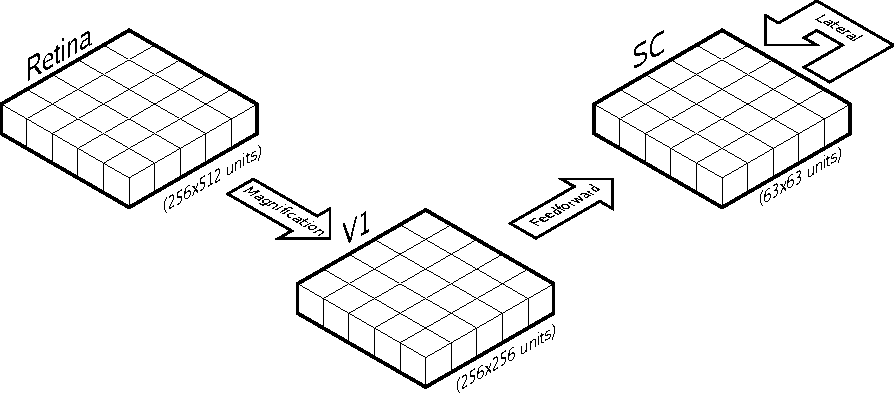
\includegraphics[width=\textwidth]{Chapitres/PublicationsSample/Chapitre/figures/model}
  \end{center}
  \caption {The model is made of three distinct groups. The retina receives
    input from a CCD camera and transmit information to the primary visual
    cortex where the actual magnification occurs. This result is then feed to
    the superior colliculus where salient locations enter competition.}
  \label{fig:model}
\end{figure}
%%
We will now detail the cortical magnification occurring between the retina and the
primary visual area V1 as well as the competition occurring within the superior
colliculus resulting in a unique localized packet of excitation designing the
selected target.

%---------------------------------------------------------------------------
\subsubsection{Cortical Magnification}
The retina represents the sensory input space and possesses a complex structure
composed of several layers of neurons. Vision actually starts early in the
layer of photo-receptors from where the flow of information is processed via
the ganglion cells which are large nerve cells whose cylindraxes form the optic
nerve. Due to the non-homogeneous repartition of photo-receptors on the (human)
retina surface, visual acuity decreases from the center of the retina (fovea)
to its periphery. This property is attributed to a variation in the density of
photo-receptors that decreases from the center to the periphery
\cite{Marilly:1999}. Consequently, the foveal region benefits from a much
higher resolution than peripheral regions and this property is preserved along
the visual pathway up to early visual areas \cite{Purves:2004}. This is
referred to as {\em cortical magnification}. To analyze this magnification in a
quantitative way, a coordinate system is often defined in the visual field. The
coordinate system that is best suited to the visual system is the polar
coordinates $(\rho,\phi)$. It characterizes a position in the visual field by
its eccentricity $\rho$ from the center of gaze and its polar angle $\phi$ is
measured, for example, in relation to the lower vertical meridian. We can
therefore define a retinotopic map which corresponds to the spatial
transformation of the image by the spatial arrangement of the grid of
neurons. It is often approximated by a log-polar transformation of the
spherical image centered on the eye \cite{Robinson:1972}. We used a simplified
model of the retina considering only the photo-receptors layer. And for
computational reasons (speed), we did not enforce the non-uniform repartition
of photo-receptors on the retina surface. Instead, we modeled a uniform
distribution of neurons onto the retina associated with a deformed polar
coordinate system as proposed by \cite{Ottes:1986}. Each cortical visual cell
is supposed to be connected to a single or several photo-receptor cells, with
respect to a logpolar deformation, that form its receptive field. So the non
uniformity is caused by the changing size of the receptive fields. We used
equations mapping retinotopic polar coordinates $(\rho,\phi)$ onto V1 Cartesian
coordinates $(\mathbf{x},\mathbf{y})$. These equations were first introduced by
\cite{Ottes:1986}:
\begin{eqnarray}
  \mathbf{x} &=& B_x \ln{(\frac{\sqrt{\rho^{2}+2A\rho|\cos{(\phi)}|+A^{2}}}{A})}\\
  \mathbf{y} &=& B_y \arctan{(\frac{\rho \sin{(\phi)}}{\rho|\cos{(\phi)}|+A})}
  \label{eq:magnification}
\end{eqnarray}
with $A=3^\circ$, $B_x=1.4mm$, $B_y=1.8mm$. These parameters have been chosen
to fit the stimulation map of the SC given by \cite{Robinson:1972}.  A neuron
in the visual cortex fires an action potential when a visual stimulus appears
within its receptive field. But for any given neuron, it may respond best to a
subset of stimuli within its receptive field corresponding to its preferred
direction. Neurons with similar tuning properties (what the neurons respond to)
tend to cluster together but the exact structure is still unclear. Then, it is
acceptable to assume that V1 has a retinotopic map similar to the collicular
motor map in \cite{Bear:1996}. It means that a cell at a given position
$(\mathbf{x},\mathbf{y})$ in the V1 map is activated by retinal cells in
positions ($\rho$, $\phi$) according to given equations. One result of this
deformation is that the same stimulus causes a large activation in the V1 map
if it is located near the fovea and smaller activation in peripheral positions
(cf. figure \ref{fig:magnification}).
\begin{figure}[htbp!]
  \centering
    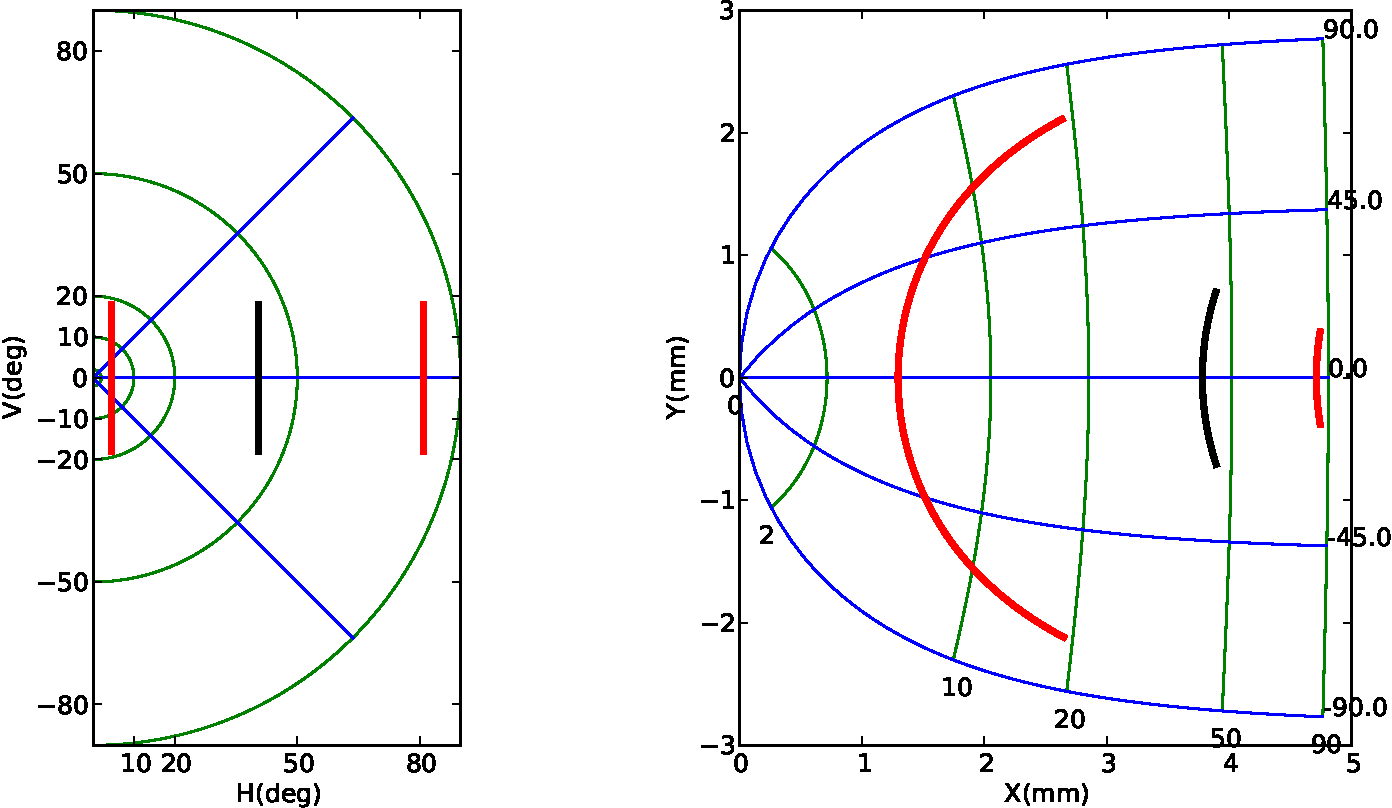
\includegraphics[width=\textwidth]{Chapitres/PublicationsSample/Chapitre/figures/mapping}
  \caption{Cortical magnification from the retina to the visual cortex distorts
    geometrical properties of the image while keeping neighborhood
    relationship.}
  \label{fig:magnification}
\end{figure}
Visual receptors of V1 have been modeled in two dimensions corresponding to an
eye visual hemifield with no connection between the different receptors.

%---------------------------------------------------------------------------
\subsubsection{Dynamic Neural Field Theory}
Collicular population (the motor layer of one superior colliculus) has been
modeled with respect to the dynamical neural field theory
\cite{Wilson:1973,Amari:1977,Taylor:1999} that describes the evolution of a
neural population using equation (see \cite{Rougier:2006} for details):
\begin{equation}
   \tau \frac{\partial u(\mathbf{x},t)}{\partial t} = -u(\mathbf{x},t) +
  \int w(\mathbf{x} - \mathbf{y}) f(u(\mathbf{y})) d\mathbf{y}\\
 + h + I(\mathbf{x}, t)
    \label{eq:dnf}
\end{equation}
where $\mathbf{x}$ denotes a location onto the SC; $t$ is time; $u(\mathbf{x},
t)$ denotes the membrane potential of a neural population at point $\mathbf{x}$
and time $t$; ${\tau}$ is the temporal decay of synapses, $f$ is a sigmoid
function computing the mean firing rate, $w$ is a neighborhood function,
$s(\mathbf{x})$ is the input received at position $\mathbf{x}$ and $h$ is the
mean neuron threshold. $w$ has been set as a difference of Gaussian ($DoG$) with
short-range excitations and long range inhibitions following anatomical and
physiological data as reported in~\cite{Munoz:1998}:
\begin{equation}
  \label{eq:DoG}
  w ({\bf x}-{\bf y}) = 
    A e^-{\frac{\vert {\bf x} - {\bf y} \vert^2}{a^2}} -
    B e^-{\frac{\vert {\bf x} - {\bf y} \vert^2}{b^2}}
\end{equation}
and $f$ has been set as a simple rectification of ${\bf x}$. The input
$I(\mathbf{x},t)$ is a direct one-to-one relationship according to V1 and SC
respective sizes.





%---------------------------------------------------------------------------
\subsection{Results}
The reported experimental results are of three kinds. Firstly, we
check that basic properties of information encoding are ensured
(topology, accuracy). Secondly, we examine the resulting saccadic
behavior for target selection from exogenous information, particularly
depending on the position of candidate targets with regard to the
fovea. Thirdly, we address more difficult cases, particularly
considering natural images and introducing the need for endogenous
information.

%---------------------------------------------------------------------------
\subsubsection{Output Decoding}
One of the questions related to the superior colliculus concerns the proper way
to decode the output. Since the amplitude and direction of a saccade depend on
the activity of the neural population in the deep SC \cite {Sparks:1990},
different ways of SC output evaluation have been proposed in the past:
\begin{itemize}
\item winner-take-all where the most active site indicates the direction
\item summation\cite{McIlwain:1976,Sparks:1976} where all activities of active
  neurons are summed with weights determined by their individual labels
\item weighted average \cite{Lee:1988} using a normalization
  according to the number of active neurons
\end{itemize}
These three evaluation schemes are equivalent in the case of a
normally activated population but differ when there is a deactivation
or an over-activation of a part of the population. We have retained
the last decoding scheme because the superior colliculus was modeled
using a dynamic neural field and it is thus ensured that a stereotyped
activity profile emerges anytime corresponding to the most salient
location of the V1 area. Furthermore, this stereotyped activity
possesses a Gaussian shaped two-dimensional profile and it is possible
to find its center of mass. We have been testing the accuracy of this
coding scheme by feeding the model with standard Gaussian shaped
stimuli at different locations (see figure
\ref{fig:accuracy}). Despite the magnification effect, one can see
that the model has a high precision in the standard saccadic range
($-30^\circ$ to $+30^\circ$, 0 to 50). We also tested the inactivation
of a subpart of the collicular layer to check that we obtain both
hypometric and hypermetric saccades as reported in
\cite{Robinson:1972} (results not presented here).
\begin{figure*}
  \centering
    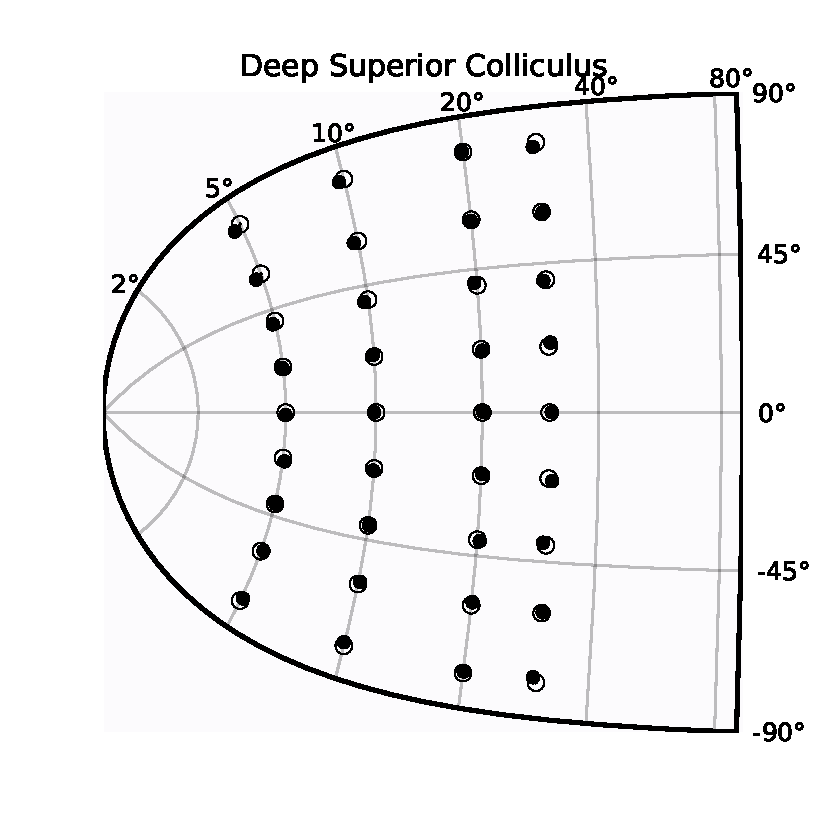
\includegraphics[width=1.0\textwidth]{Chapitres/PublicationsSample/Chapitre/figures/accuracy}
  \caption{Accuracy of the model of the superior colliculus has been measured
    using a set of retina targets that have been
    sequentially presented to the SC model. For each target and after
    convergence (difference of activity between time $t$ and time $t+dt$ is
    negligible), the center of mass of the collicular activity has been decoded
    and represented as a circle (black dots represent the
    actual projection of the target in collicular coordinates).}
  \label{fig:accuracy}
\end{figure*}

\subsubsection{Target Selection from exogenous information}

Several studies have provided data on the organization of the saccadic
path \cite{Yarbus:1967,Levy:1974,Noton:1971}. A set of
experiences on adults with normal vision showed that the attractive
value of a visual stimulus depends strongly on its distance relative
to the previous fixation point (short distances preferred). Moreover,
for several targets at the same distance, this attractive value is
greater when the eccentricity is less important (targets closer to the
fovea preferred). This result can be interpreted in the purposive
framework evoked above, associating vision and preparation for
action. In this perspective, shorter saccades are preferred and a
nearby object is more interesting than a distant object for example in
the case of hunger or danger.

Interestingly, our model displays a similar behavior and provides an
explanation that is based on the topology of the neural network
preparing the saccade. On the one hand, the spatial distribution of
collicular neurons and their receptive fields resulting from the
log-polar transformation (cortical magnification) reflect in a
qualitative way how the visual information is transformed from the
retina to the motor map of the superior colliculus. A visual stimulus
projected onto the foveal region evokes more neural activity (on the
rostral part of the collicular map) than a similar stimulus in the
peripheral region.  On the other hand, the connectivity of the DNF
model plays the role of a "winner-take-all". The profile of inhibition
ensures that the system reaches a stable state once a neighborhood is
recruited; there is always a selection at the end of the process. But
this selection made at the premotor level does not always reflect a
sensory selection: In some cases, the recruited population corresponds
to an averaging and the final target may be a position where there is
no stimulus; this depends on the profile of the lateral connections.
Figure \ref{fig:selection} reports an experiment where the model is
tested using two punctual equivalent stimuli (same aperture, intensity
and shape).  Their attractive value is estimated in V1 map.  The
cortical population activated by the stimulus at $3^\circ$ is larger
than the population activated by the stimulus at $10^\circ$. Then, the
resulting activity after computation in the deep layer of the superior
colliculus is a stable bubble in the first position. So it can be said
that the selection of the nearby stimulus emerges from the local
computation.

\begin{figure}
  \centering
    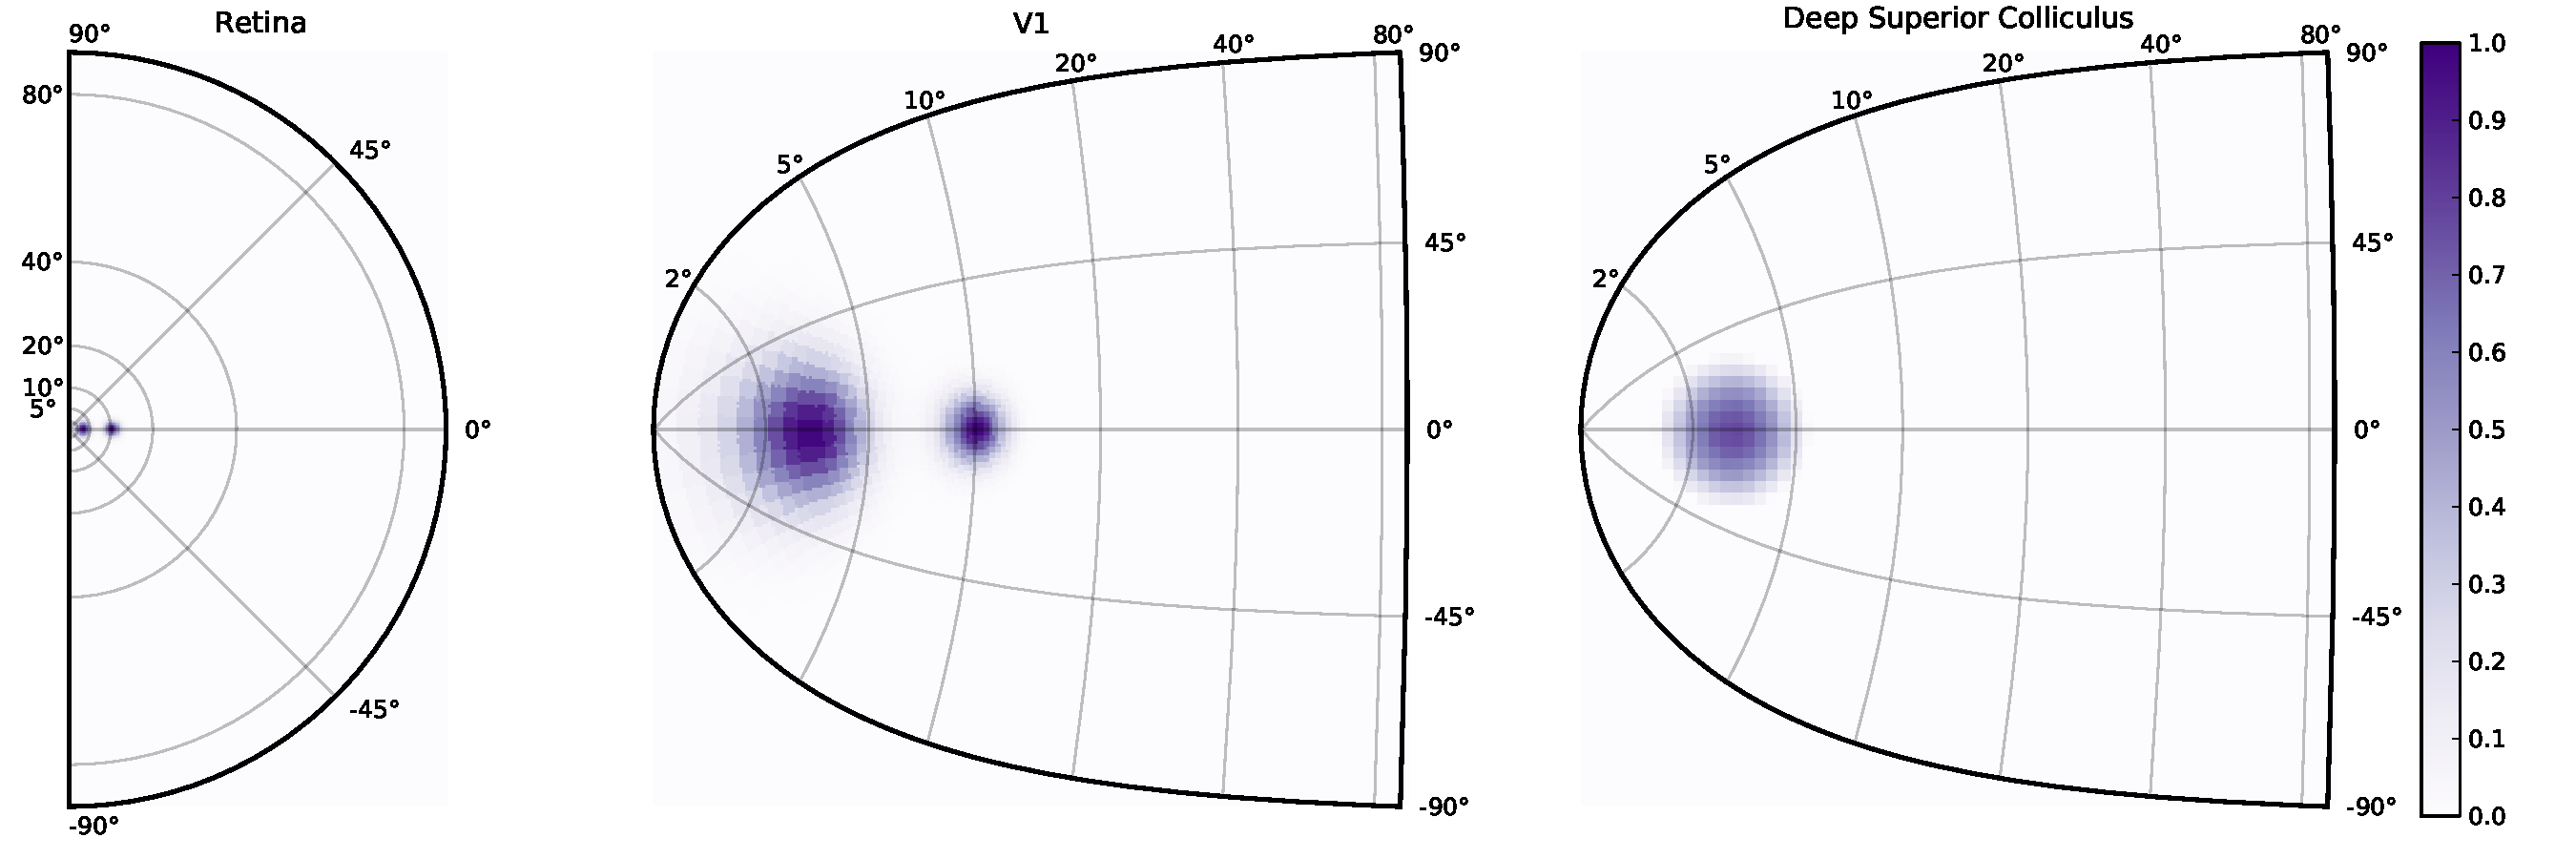
\includegraphics[width=\textwidth]{Chapitres/PublicationsSample/Chapitre/figures/selection}
  \caption{The projection of two equivalent horizontal stimuli but at different eccentricities. The stimulus nearer to the fovea is automatically selected to be the saccade target. }
  \label{fig:selection}
\end{figure}

%---------------------------------------------------------------------------
\subsubsection{Natural Images Processing}
We have also tested the model using natural images taken from a color CCD
camera. No image processing has been performed on the image but a conversion to
a gray-level representation. Figure \ref{fig:colliculus} exhibits an example
where a subpart of a computer keyboard has been shot. This allows to illustrate
the main feature of the proposed model. If one look closely at the half retina
representing the keyboard (upper left part of the figure), one can see that
several letters ({\tt O, P, L, M}) are eligible for attention focus and for
ocular saccade. However, the retinotopic projection onto the model of the V1
area reduces quite naturally this set to letters {\tt O} and {\tt L}.
\begin{figure*}
  \centering
    \includegraphics[width=1.0\textwidth]{Chapitres/PublicationsSample/Chapitre/figures/colliculus-1}\\
    \includegraphics[width=1.0\textwidth]{Chapitres/PublicationsSample/Chapitre/figures/colliculus-2}
  \caption{An image of a computer keyboard has been captured using a color
    camera (resolution $1024 \times 1280$) and transformed into a normalized
    gray level image. \textbf{Upper figure.} The right half of the image is
    presented to the half retina area which in turn feeds the V1 area where
    retinotopy is applied following equation \ref{eq:magnification}. The
    colliculus area enters a competition stage where most salient locations are
    eligible for final activation and after some iterations, the competition
    ends up onto the {\tt O} letter that is thus considered the most salient
    location of the visual scene according to its location and
    activation. \textbf{Lower figure.} A saccade has been simulated to center
    the {\tt O} letter into the center of the fovea and the colliculus now
    focuses onto a subpart of the {\tt O} letter that appears to be the newly
    most salient location of the new visual scene.}
  \label{fig:colliculus}
\end{figure*}
The model of the SC is thus confronted with a choice between these two
locations and the dynamic field theory, as it has been introduced in the
previous section, ensures that only one location remains after
competition. However it is hard to specify the exact conditions that make the
model focus on the {\tt O} instead of the {\tt L} letter in the given
example and the spatially compact shape of the {\tt O} is certainly to be taken
into account. This example also underlies the inherent difficulty in temporally
organizing ocular saccades without any top-down control. If we were to let the
model only react to its sensory input, it would certainly focus on the most
salient location without ever exploring other points of interest (from a
behavioral point of view). If the actual saccade brings into view another
salient location, the model would jump again to the new location (provided we
inhibited the foveal region to prevent the model to be stuck forever on this
single location) but in such a case, nothing would prevent the model from going
to location A then location B and then again location A, being trapped in a
cycle. Exploring the whole visual scene thus requires some kind of top down
control to be able to dynamically inhibit visited location once they have been
focused in order to favor other locations. This is out of scope of the present
article but this has been already made in a wider but less realistic model
\cite{Fix:2006}.



\subsection{Discussion}
We have introduced in this paper a model of the superior colliculus based on on
a large set of biological data. This model has been designed using a strongly
constrained modeling framework relying on a set of four computational
principles (distributed, asynchronous, numerical and adaptive) and those
properties ensure to some extent that the model does not suffer from usual
artifacts of such computational framework (presence of a central supervisor
deciding of the actual behavior). More specifically, the saccadic behavior we
exhibited through the various experiments is a true and emergent property of
local and homogeneous computations only. If we give a closer look to the
selection process that is carried out when the model is presented with two
identical stimuli (but at two different locations), we may explain the
selection of the stimuli closest to the foveal region because of the cortical
magnification. Said differently, the cortical magnification deeply influences
the network topology and consequently the saliency of any presented stimuli. If
we were to use some different magnification function, this would modify as well
the selection process. This selective behavior is thus tightly linked to the
spatial and physic implementation of the computational units. The intelligence
of the system is thus rooted in its physical instantiation (even though it is
simulated in our case).\\

However, if we now give a closer look to figure \ref{fig:magnification}, we may
realize that there is counterpart for such an automatic selection. Because the
foveal region benefits from a much higher resolution than peripheral regions,
the projections from retina to the V1 region distorts the geometrical
properties of the image. This is especially the case of straight lines that are
now projected as curved lines within the V1 region. Furthermore, the projection
of any straight line from retina to V1 is unique and does not benefit from the
same geometrical properties. How do we recognize a straight line in such
conditions ? Classical answers relying on generic neighborhood functions that
would (for example) link geometrically {\em aligned} neurons (hence mimicking
the abstract description of a geometrical line) is not possible anymore. We
thus have to change paradigm and consider new approaches like the one described
in \cite{ORegan:2001}. In this article, authors propose to reconsider vision by
integrating the sensory-motor dimension of perception. Even though a straight
line is not projected as a straight line in visual regions, there is
nonetheless a physical property that remains true independently of the physical
apparatus: if we move eyes along a straight line, there is an invariance in the
projection because this is the physical definition of a line. Such
sensori-motor behavior is a complex challenge that we are now actively
exploring in terms of the temporal organization of the saccadic behavior. In
order to achieve such active behavior, we now have to consider endogenous
inputs conveying such information as instructions, goals or motivations from
other higher-level neural structures. This lead us to consider anatomical
structure such as the basal ganglia that are known to be deeply involved with
voluntary motor control. In the end, we expect the model to achieve vision and
recognition based on motor learning that may ultimately replace {\em passive
  perception}.





